\documentclass[UTF8,11pt,a4paper]{ctexart}
\usepackage[top=2.1cm,bottom=2.1cm,left=2.3cm,right=2.3cm]{geometry}
\usepackage{graphicx,booktabs,array,longtable,amsmath,amssymb,xcolor,hyperref,fancyhdr,setspace}
\graphicspath{{lai_figures/}}
\hypersetup{colorlinks=true,linkcolor=blue,urlcolor=blue}
\setstretch{1.18}
\setlength{\parindent}{2em}
\setlength{\parskip}{0.35em}
\pagestyle{fancy}
\fancyhf{}
\fancyhead[L]{\small JIIM 对标论文中文译读版}
\fancyhead[R]{\small\thepage}
\renewcommand{\headrulewidth}{0.4pt}

\definecolor{notegray}{RGB}{245,247,249}
\newcommand{\transnote}[1]{\begin{center}\fcolorbox{gray}{notegray}{\parbox{0.92\textwidth}{\small #1}}\end{center}}

\title{使用 StyleGAN2-ADA 生成脑 MRI：\\训练集规模对合成图像质量的影响}
\author{原作者：Matteo Lai、Mario Mascalchi、Carlo Tessa、Stefano Diciotti\\中文译读版整理：基于 CC BY 4.0 授权版本}
\date{原文在线发表：2025年9月23日\\\href{https://doi.org/10.1007/s10278-025-01536-0}{DOI: 10.1007/s10278-025-01536-0}}

\begin{document}
\maketitle

\transnote{\textbf{版权与版本说明：}本文件是原论文的中文非官方译读版，旨在帮助理解 \textit{Journal of Imaging Informatics in Medicine} 的论文结构和实验表达。原文由 Springer Nature 以 Creative Commons Attribution 4.0 International（CC BY 4.0）许可发布。本文在翻译过程中进行了中文排版重组，并对部分术语保留英文缩写。若译文与原文存在差异，以英文正式版本为准。许可链接：\url{https://creativecommons.org/licenses/by/4.0/}。}

\begin{abstract}
医学影像领域的深度学习潜力经常受到数据可用性不足的限制。生成模型可以产生复现真实数据统计特征、同时更便于共享的合成数据，从而缓解这一问题。本研究考察训练集规模对先进生成对抗网络 StyleGAN2-ADA 性能的影响。模型使用 OpenBHB 数据集中的 3,227 名受试者训练，用于生成健康受试者脑 MRI 的二维切片。研究通过定性评价和当前常用的定量指标评估合成图像质量，并将相关评价工具公开发布。

结果表明，StyleGAN2-ADA 能够生成逼真且高质量的图像，甚至可使专业放射科医师难以区分真伪；同时模型未记忆训练图像，因而表现出良好的泛化和隐私保护特征。增加训练集规模只轻微改善保真度指标，对多样性指标没有明显影响，说明模式崩溃仍然存在。此外，覆盖率和 $\beta$-召回率等多样性指标对参与计算的合成图像数量高度敏感：当合成图像数量显著多于真实图像时，这些指标可能被高估。因此，必须谨慎解释多样性指标，并结合互补评价方法进行稳健评估。总体而言，StyleGAN2-ADA 具备生成隐私友好型医学合成图像的潜力，但要克服多样性不足，仍需探索替代生成架构或加入新的正则化策略。
\end{abstract}

\noindent\textbf{关键词：}脑 MRI；生成对抗网络；医学影像；合成数据

\section{研究背景}

深度学习技术有望通过个体化诊断和影像生物标志物发现推动医学影像研究。然而，医学数据的可用性受到隐私问题、采集成本和采集时间等多方面限制。缓解数据不足的常用策略是数据增强，但增强样本通常与原始数据高度相关。另一种方法是利用生成模型产生合成数据。生成模型旨在学习并复现观测数据的统计性质，从而建立合成数据分布。高质量合成数据既可能支持与真实数据相近的分析，也可能降低隐私泄露风险，有助于数据共享、开放科学和研究加速。

在医学图像生成领域，生成对抗网络（GAN）和扩散模型是两类重要方法。两者都能生成高质量图像，但扩散模型可能复制或过拟合训练样本，而 GAN 常受到模式崩溃影响，无法覆盖真实数据分布的全部多样性。由于二者均依赖深度网络训练，其性能也会受到训练数据规模影响。

本研究关注 Karras 等提出的 StyleGAN2-ADA。该模型通过自适应判别器增强（adaptive discriminator augmentation, ADA）优化小数据集训练。ADA 根据过拟合启发式指标动态调整增强强度，并使用不会泄漏到生成图像的增强操作。StyleGAN2-ADA 还通过判别器中的小批量标准差归一化和生成器中的逐像素特征向量归一化缓解模式崩溃。前者鼓励模型在小批量层面匹配真实与生成数据的变化，后者限制对抗竞争过程中生成器和判别器内部特征幅度的无界增长。

StyleGAN2-ADA 被认为是性能较强的 GAN 架构之一，也已用于多类医学影像任务，尤其适合有限数据场景。然而，其可靠性同时取决于训练数据规模和评价方法的严谨程度。原始 StyleGAN2-ADA 工作分析过训练集规模，但主要使用 Fr\'echet Inception Distance（FID）进行评价。Zoghby 等进一步研究了 pix2pix GAN 在脑 MRI 图像到图像转换中的训练集规模效应，发现较小数据集也可能获得接近较大数据集的表现；不过，该研究的受试者多样性和评价指标维度仍然有限。

合成图像评价本身也是关键问题。FID 将保真度和多样性压缩为单一分数，不能覆盖生成质量的所有维度。PSNR、NMSE 和 SSIM 等逐图像指标虽然广泛用于脑 MRI 评价，却无法描述真实数据与合成数据之间更广泛的分布关系。更稳健的评价框架应分别考察：保真度，即合成数据的真实感；多样性，即对真实数据分布的覆盖程度；以及泛化性，即是否生成新的而非记忆的样本。

基于上述空白，本研究使用多维评价框架分析训练集规模对 StyleGAN2-ADA 的影响。作者将不同文献中的评价指标整合到公开 GitHub 工具库中，使其能够迁移到其他数据集和模态。研究使用 OpenBHB 数据集的脑 MRI 二维切片，分别构建 1,000、2,000 和 3,227 张图像的训练集，并从保真度、多样性和泛化性三个角度开展定量与定性评价。

\section{研究方法}

\subsection{数据来源与预处理}

研究使用 OpenBHB 数据集。该数据集汇集 10 个公开数据集中的健康受试者 T1 加权脑 MRI，包括 3,227 张训练图像和 757 张验证图像。作者保留原数据划分，并将 757 张验证图像作为独立测试集。

OpenBHB 提供 CAT12、FSL 和 quasi-raw 三类预处理版本。研究选择经过最少预处理的 quasi-raw 图像，以尽量保留 MRI 的原始特征。该流程包括：使用 ANTs 进行偏置场校正；使用 FSL FLIRT 将图像以 9 个自由度仿射配准到 $1\,\mathrm{mm}^3$ MNI 模板，并避免剪切变换；应用脑掩膜去除非脑组织。

随后，每个体数据被归一化到 $[0,1]$，提取尺寸为 $182\times218$ 像素的中央轴位切片，得到每名受试者一张二维图像。图像经零填充扩展为 $256\times256$，并合并为尺寸 $256\times256\times N$ 的 NIfTI 数据，其中 $N$ 为图像数量。

\subsection{模型训练}

研究采用 StyleGAN2-ADA 官方 PyTorch 实现，并沿用 Karras 等提出的默认超参数，仅删除不适用于灰度 MRI 的亮度翻转、色相旋转和饱和度等颜色增强。模型分别使用 1,000、2,000 和完整 3,227 张图像训练，以分析数据规模的影响。每个模型训练 2,200 kimgs，即累计处理 220 万张批次图像。所有训练均在单张 NVIDIA A100 GPU 上完成，每个配置约需 25 天。

\subsection{定量评价框架}

作者将指标分为保真度、多样性和泛化性三类，如图~\ref{fig:metric} 所示。由于不存在能够单独覆盖所有质量维度的指标，研究将既有实现整合为统一工具库，并设计两类比较：

\begin{enumerate}
\item \textbf{训练集对齐：}将合成图像与 3,227 张训练图像比较，评价保真度、多样性和训练数据记忆。分别使用 50,000 张合成图像，以及与真实训练集规模接近的 3,000 张合成图像。
\item \textbf{未见数据一致性：}将合成图像与 757 张独立测试图像比较，评价对分布外样本的稳健性和一致性。分别使用 50,000 张合成图像，以及与测试集规模接近的 700 张合成图像。
\end{enumerate}

\begin{figure}[htbp]
\centering
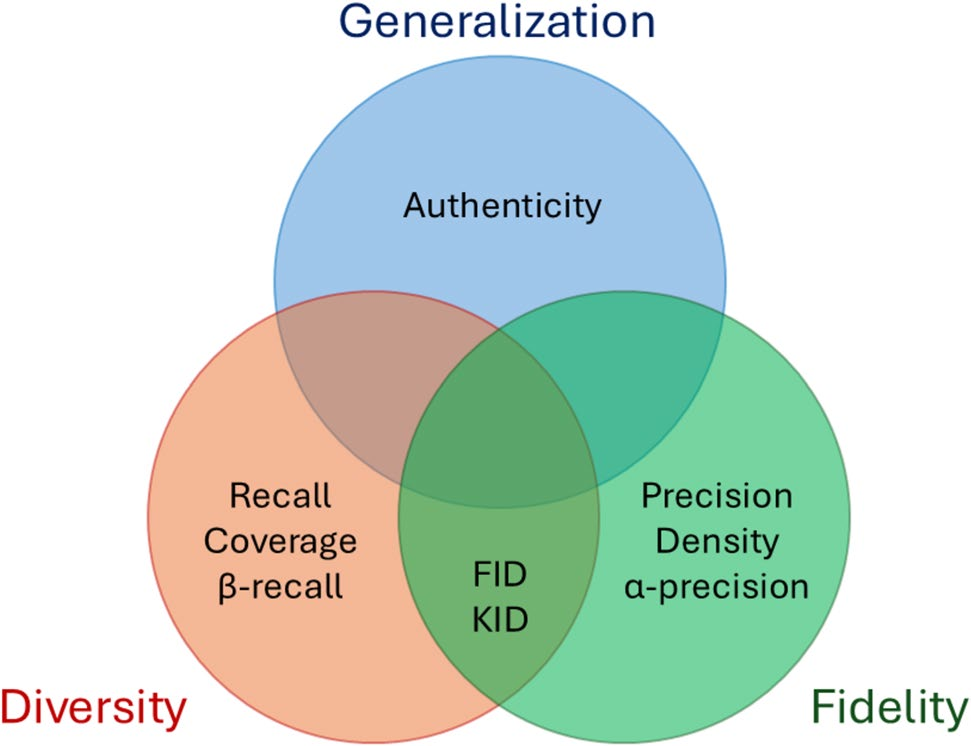
\includegraphics[width=0.66\textwidth]{fig-000.jpg}
\caption{评价指标被划分为泛化性、多样性和保真度三个维度。FID 和 KID 同时反映保真度与多样性；Authenticity 评价泛化性。图源：Lai et al.，CC BY 4.0。}
\label{fig:metric}
\end{figure}

\subsubsection{Fr\'echet Inception Distance}

FID 在 Inception 网络特征空间中，将真实和合成数据分布近似为高斯分布，并计算二者的 Fr\'echet（Wasserstein-2）距离。FID 越低表示分布越接近。它同时受到保真度和多样性影响，是生成图像评价的常用指标；但其数值会受到参与计算的图像数量影响。

\subsubsection{Kernel Inception Distance}

KID 使用多项式核估计真实与合成特征分布的差异，被视为 FID 的无偏替代指标。与 FID 类似，KID 同时反映保真度和多样性，数值越低越好。

\subsubsection{Precision 与 Recall}

Precision 和 recall 使用预训练 VGG-16 的特征空间，分别量化保真度和多样性。真实与合成样本通过第 $k$ 近邻特征向量定义为流形。Precision 统计生成样本落入真实数据流形的比例，用于衡量合成图像的真实感；recall 统计真实数据流形被生成模型覆盖的比例，用于衡量生成多样性。两者取值范围为 $[0,1]$，越高越好。

\subsubsection{Density 与 Coverage}

Density 和 coverage 用于缓解传统 precision/recall 对离群点的敏感性。Density 计算一个合成样本被多少个真实样本邻域球覆盖，用于评价保真度；coverage 计算至少包含一个合成样本的真实样本邻域比例，用于评价多样性。两者越接近 1 越好。

\subsubsection{$\alpha$-Precision、$\beta$-Recall 与 Authenticity}

$\alpha$-precision 和 $\beta$-recall 通过一类分类器将 Inception V3 特征映射到超球面，使典型样本靠近中心、离群样本靠近边界。算法逐步改变“典型样本”的阈值，并以曲线下面积分别评价保真度和多样性，得分越高越好。

Authenticity 用于评价合成数据是否记忆训练样本。真实和合成图像首先进入同一特征空间。若某个合成样本比任意其他真实样本更接近某个真实图像，该真实图像被认为可能被模型记忆。Authenticity 范围为 $[0,1]$，越高说明泛化越好。本研究按与真实数据相同大小的合成批次进行计算，直至覆盖 50,000 张合成图像，并取批次平均值。

\subsection{定性评价}

定性评价同样围绕保真度、多样性和泛化性展开。

\textbf{保真度：}两名分别具有 35 年和 30 年经验的专家参加视觉 Turing 测试。每轮随机呈现 100 张图像，其中 50 张真实、50 张合成；观察者需要判断每张图像是真实还是合成，但不知道两类样本数量相等。三个训练集规模分别进行测试，并允许观察者调整窗宽和窗位。根据真实阳性（TP）、假阴性（FN）、真实阴性（TN）和假阳性（FP），计算准确率、敏感度和特异度：

\begin{equation}
\mathrm{Accuracy}=\frac{TP+TN}{TP+TN+FP+FN},
\end{equation}
\begin{equation}
\mathrm{Sensitivity}=\frac{TP}{TP+FN},\qquad
\mathrm{Specificity}=\frac{TN}{TN+FP}.
\end{equation}

\textbf{多样性：}使用 t-SNE 将真实和合成图像投影到二维空间。作者将 3,227 张训练图像与完整训练集模型生成的 5,000 张图像比较，并在 757 张独立测试图像上重复分析。

\textbf{泛化性：}使用预训练 VGG-16 提取真实和合成图像特征，计算每张真实图像与 50,000 张合成图像的余弦相似度。对每张真实图像选择最相似的 4 张合成图像，并展示相似度最高的两组真实图像及其近邻，以检查模型是否复制训练数据。

\section{研究结果}

\subsection{视觉 Turing 测试}

表~\ref{tab:turing} 汇总两位专家在三个训练集规模下的分类结果。总体准确率为 0.43--0.55，接近随机判断，说明真实和合成图像对专家而言较难区分。训练集规模没有表现出稳定的单调影响。

\begin{table}[htbp]
\centering
\small
\caption{视觉 Turing 测试结果。每位专家在每个训练集规模下判断 50 张真实和 50 张合成图像。}
\label{tab:turing}
\setlength{\tabcolsep}{4pt}
\begin{tabular}{ccccccccc}
\toprule
观察者 & 训练集 & TP & FP & TN & FN & 准确率 & 敏感度 & 特异度\\
\midrule
1 & 1,000 & 36 & 33 & 17 & 14 & 0.53 & 0.72 & 0.34\\
1 & 2,000 & 36 & 31 & 19 & 14 & 0.55 & 0.53 & 0.38\\
1 & 3,227 & 32 & 31 & 19 & 18 & 0.51 & 0.64 & 0.38\\
2 & 1,000 & 18 & 24 & 26 & 32 & 0.44 & 0.32 & 0.52\\
2 & 2,000 & 26 & 33 & 17 & 24 & 0.43 & 0.52 & 0.34\\
2 & 3,227 & 29 & 31 & 19 & 21 & 0.48 & 0.58 & 0.38\\
\bottomrule
\end{tabular}
\end{table}

\begin{figure}[htbp]
\centering
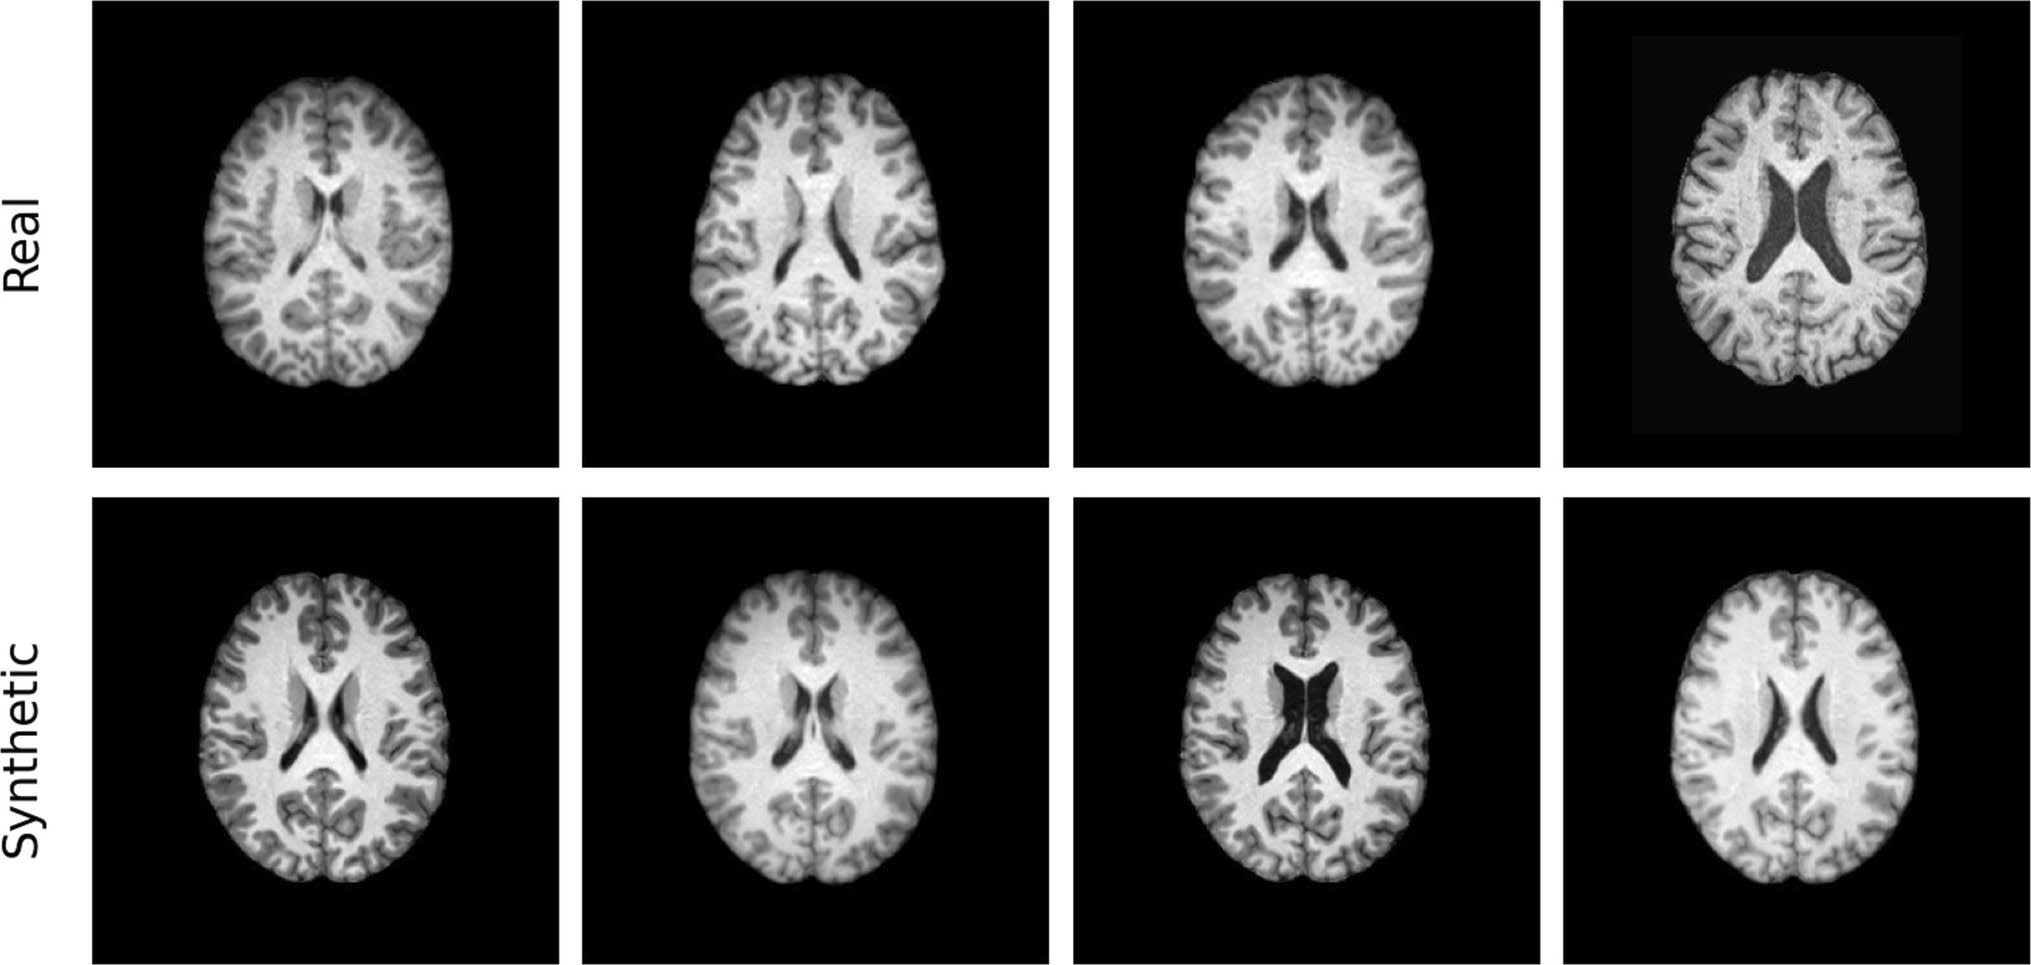
\includegraphics[width=0.9\textwidth]{fig-001.jpg}
\caption{真实图像与合成图像比较。原图上排为合成图像、下排为真实图像。图源：Lai et al.，CC BY 4.0。}
\label{fig:real-synth}
\end{figure}

\subsection{定性多样性与泛化性}

k-NN 分析显示，与真实图像最相似的合成样本仍与其近邻存在可见差异，提示模型生成的是新样本而非直接复制训练图像。然而，t-SNE 可视化显示合成图像没有覆盖完整的真实数据嵌入空间，提示模型存在多样性不足和模式崩溃。

\begin{figure}[htbp]
\centering
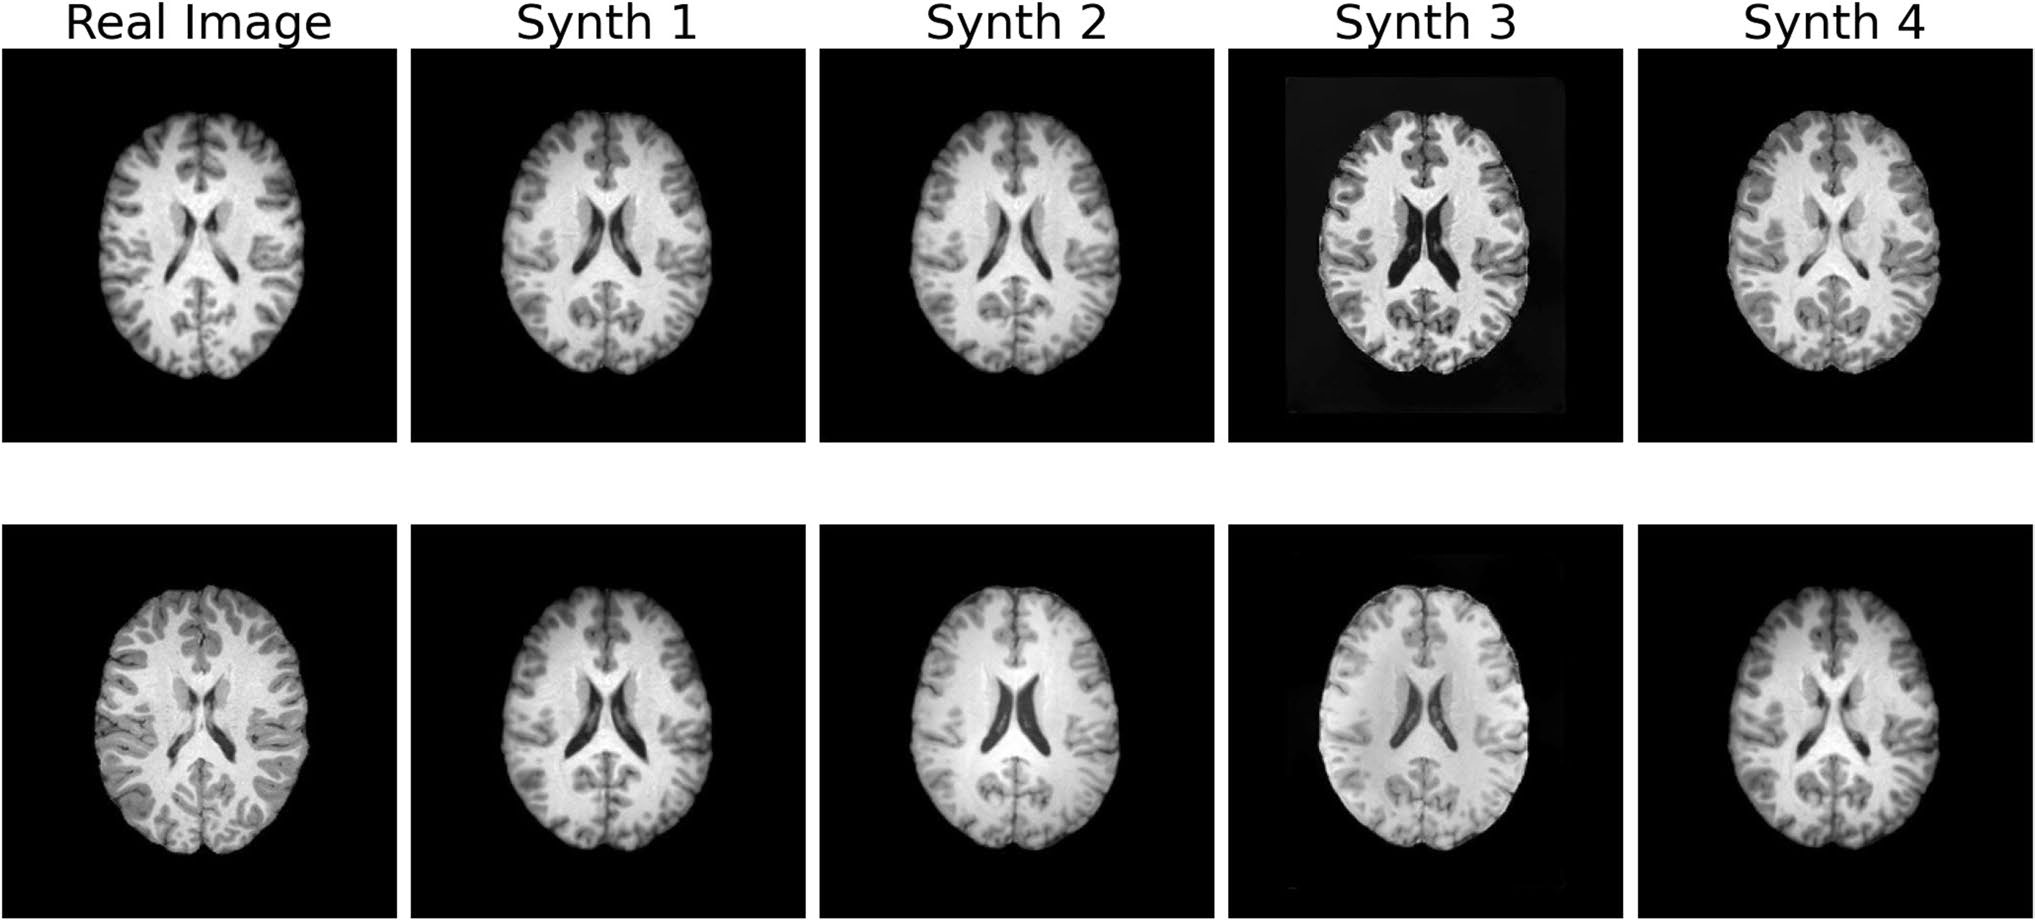
\includegraphics[width=0.92\textwidth]{fig-002.jpg}
\caption{k-NN 分析。第一列为与任意合成样本余弦相似度最高的两张真实图像，后四列为各自最相似的四张合成图像。图源：Lai et al.，CC BY 4.0。}
\label{fig:knn}
\end{figure}

\begin{figure}[htbp]
\centering
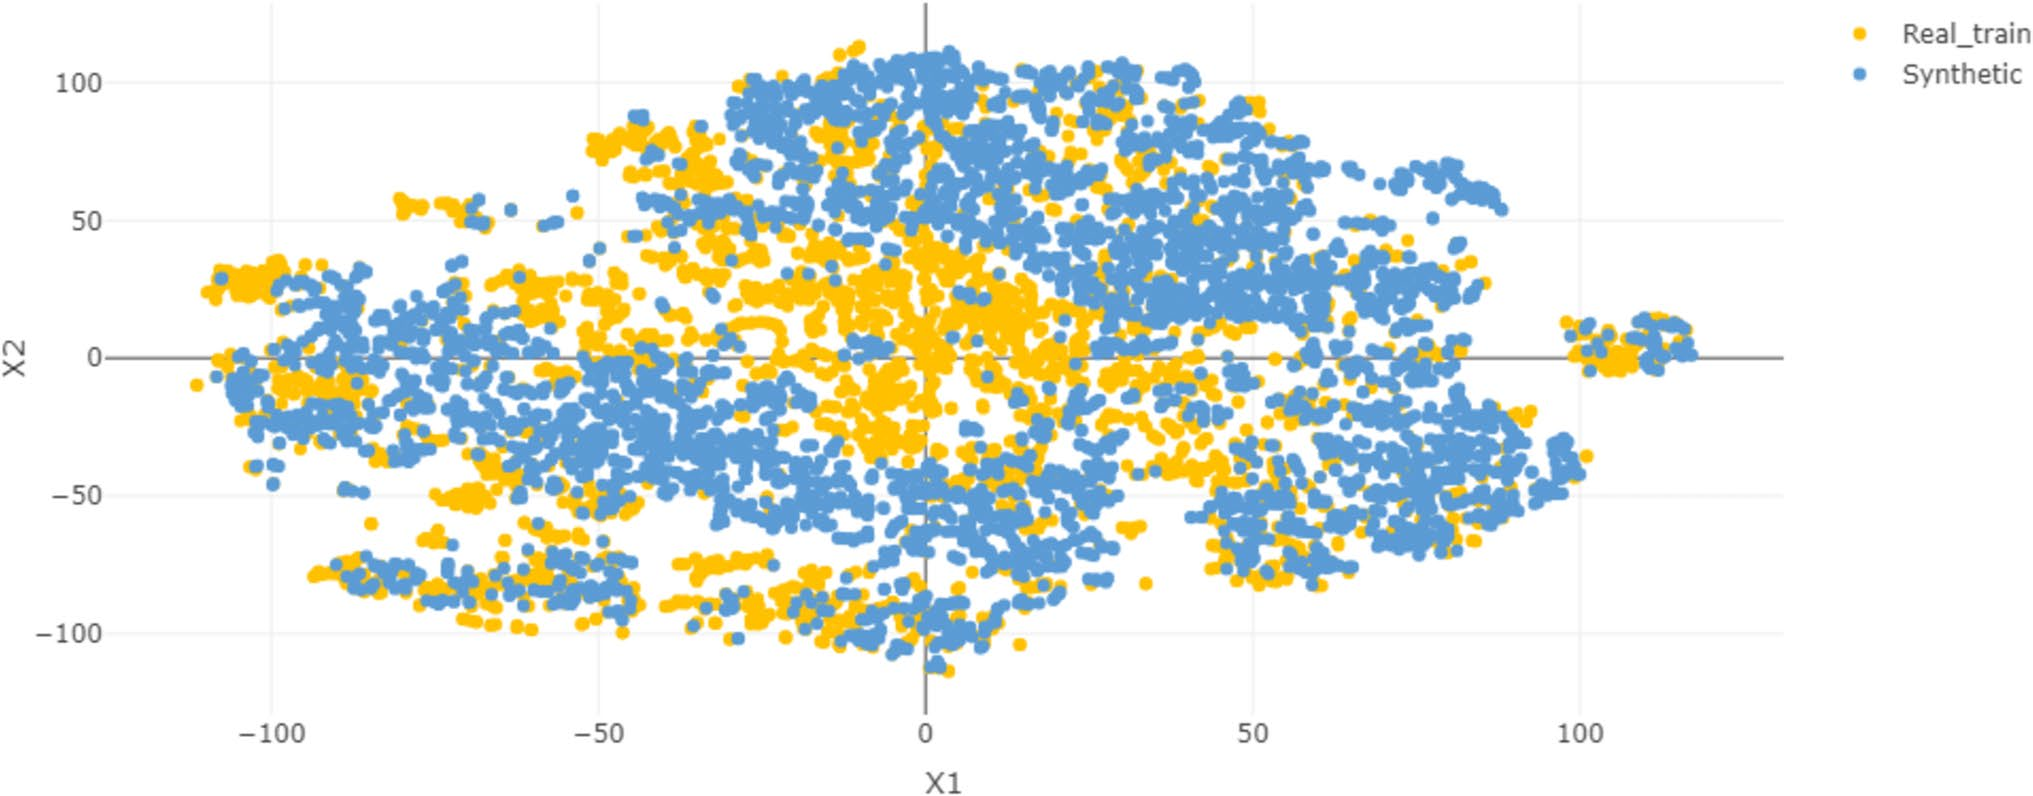
\includegraphics[width=0.86\textwidth]{fig-003.jpg}
\caption{5,000 张合成图像与全部真实训练图像的 t-SNE 可视化。真实数据与合成数据的嵌入空间仍存在未充分覆盖的区域。图源：Lai et al.，CC BY 4.0。}
\label{fig:tsne}
\end{figure}

\subsection{定量评价总体结果}

作者在三个训练集规模下，将合成图像分别与训练集和独立测试集比较。定量结果与定性观察一致：StyleGAN2-ADA 生成的图像具有较高真实感且未明显记忆训练数据，但多样性有限。较大训练集使部分保真度指标略有改善，而多样性指标没有稳定提高。

当使用相同真实图像、但把合成图像数量从 50,000 减少到 3,000 时，coverage 等指标明显下降。测试集实验也显示，$\beta$-recall 和 coverage 会随着合成样本数量变化。这说明某些多样性指标可能在合成图像远多于真实图像时被人为抬高，比较不同研究时必须控制样本数量。

\begin{figure}[htbp]
\centering
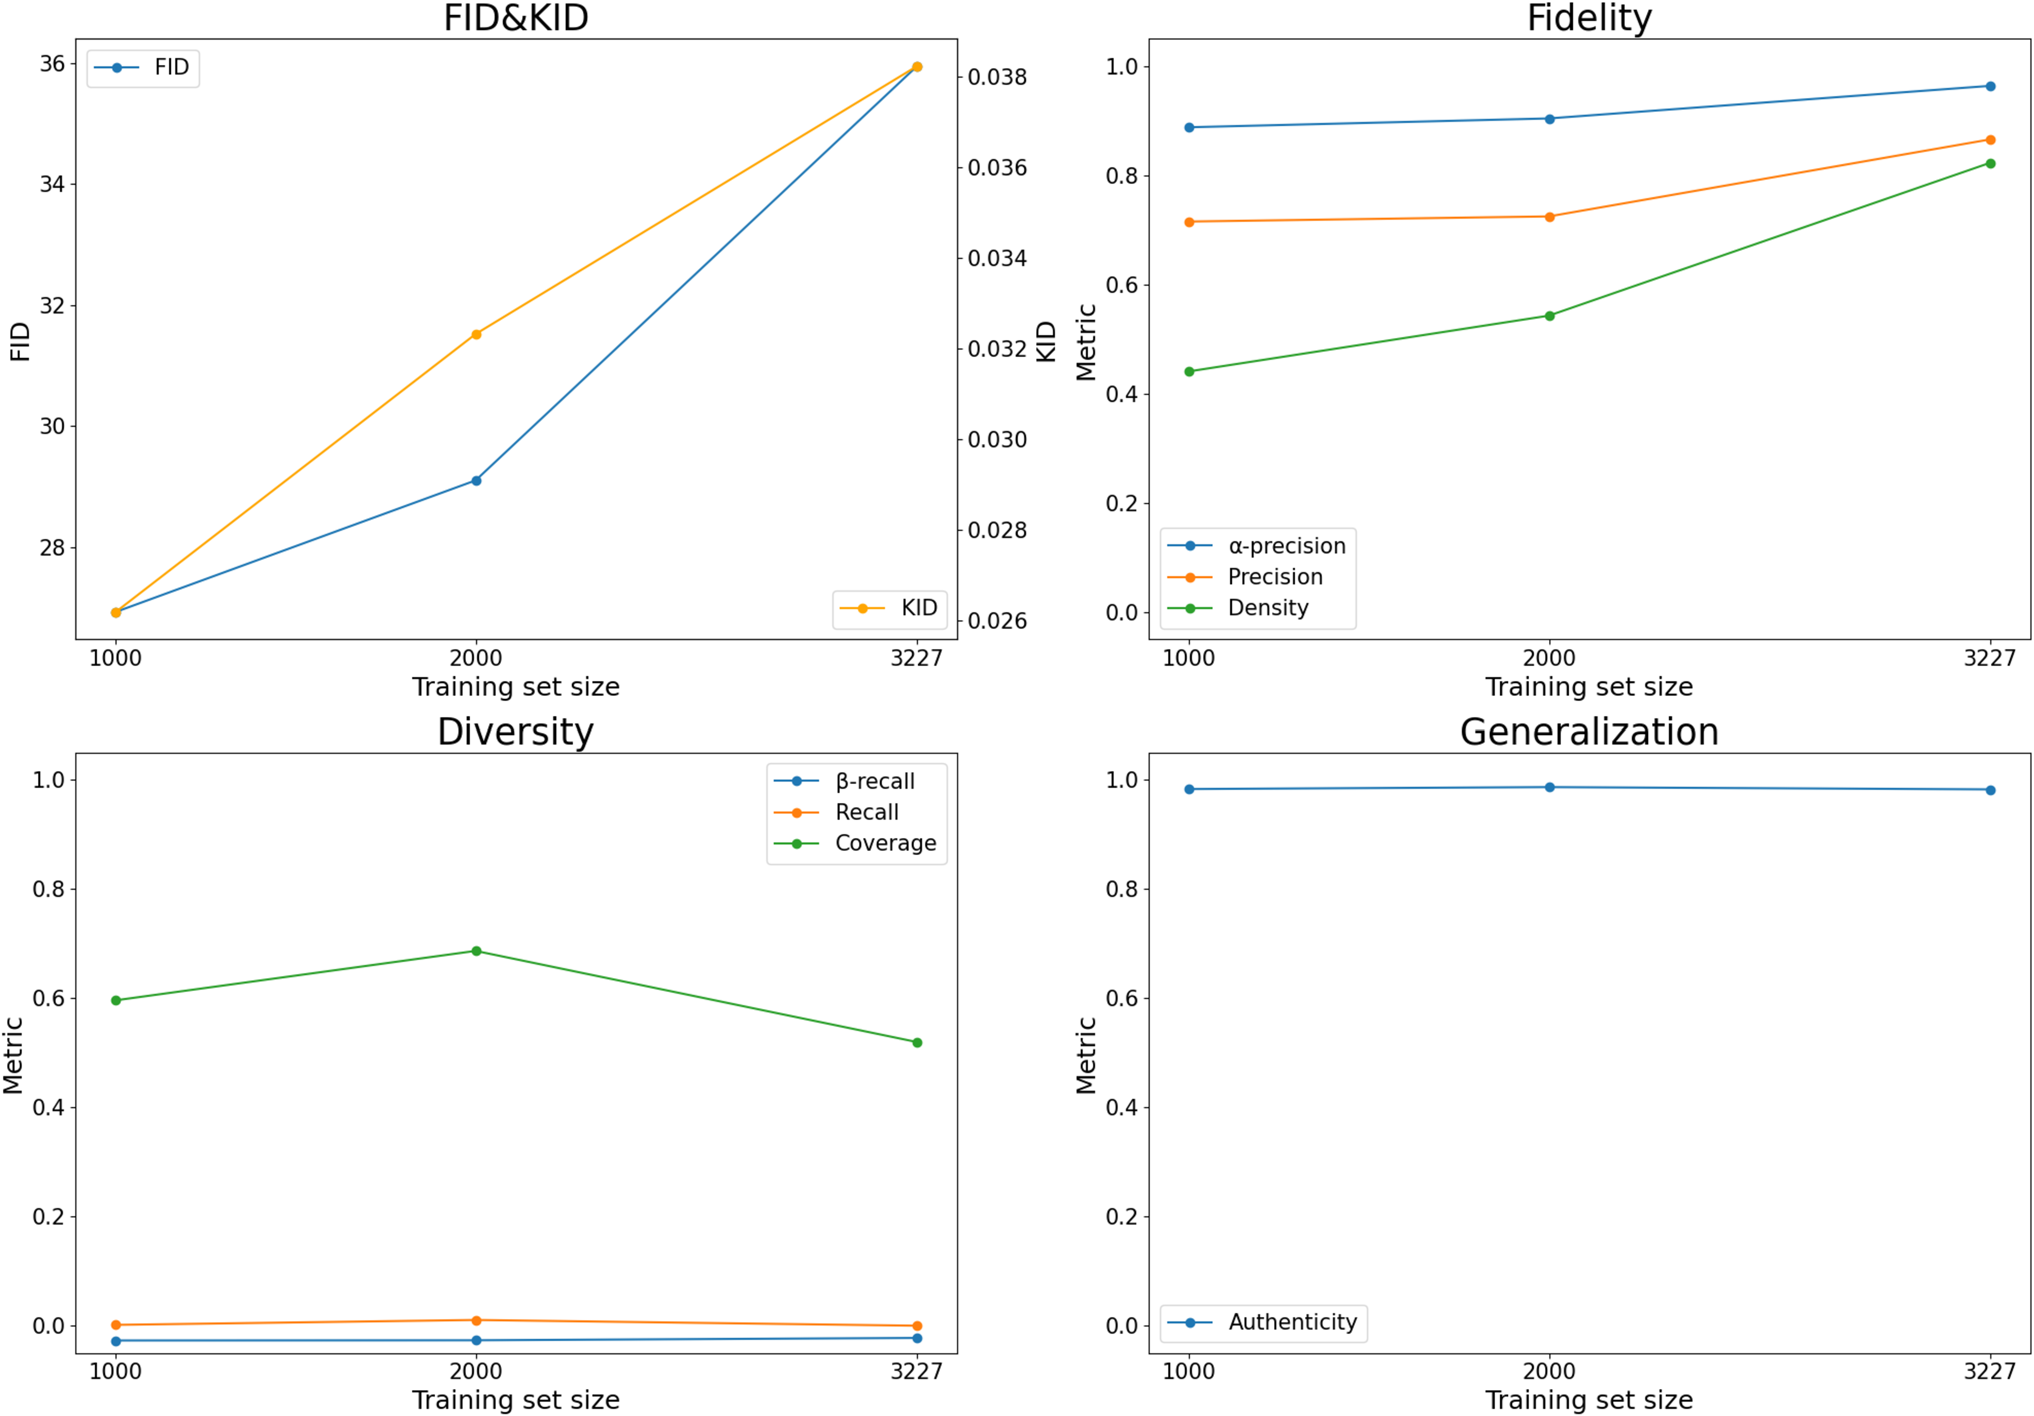
\includegraphics[width=0.95\textwidth]{fig-004.png}
\caption{不同训练集规模下的定量指标。左上：FID/KID；右上：保真度指标；左下：多样性指标；右下：泛化性指标。图源：Lai et al.，CC BY 4.0。}
\label{fig:metrics}
\end{figure}

\section{讨论}

\subsection{训练集规模的影响}

研究比较 1,000、2,000 和 3,227 张训练图像后发现，训练集规模对合成图像总体质量的影响较小。该结论与 Zoghby 等关于脑 MRI 图像到图像转换的观察一致，尽管本研究考察的是从学习分布中生成全新图像的无条件合成。较大训练集使部分保真度指标略有改善，但两位专家在视觉 Turing 测试中的准确率始终接近随机水平。

多样性指标在三个训练集规模下持续偏低，提示模式崩溃不会仅因增加训练数据而消失。相比之下，即便只使用 1,000 张训练图像，泛化指标仍然较好，说明 StyleGAN2-ADA 的自适应判别器增强可以在有限数据下抑制明显过拟合。作者据此认为，StyleGAN2-ADA 能在小数据条件下产生真实且非记忆的图像，但其内部缓解模式崩溃的机制不足以覆盖真实数据分布的全部变化。

FID/KID 与专门保真度指标之间的表面不一致，可能受到生成多样性不足影响。因此，不能只用单个综合指标判断生成模型性能，而应结合领域相关的保真度、多样性和泛化性评价。

\subsection{FID 与 KID}

三个训练集规模下，FID 为 26.92--35.94，KID 为 0.026--0.038。当用于计算的合成图像数量减少时，两者略有上升；当真实图像数量从训练集规模降低到测试集规模时，两者上升更明显。这种样本量敏感性说明，FID/KID 在不同评价设置之间并不总能直接比较，应与领域特异指标结合使用。

\subsection{保真度}

视觉观察显示，StyleGAN2-ADA 生成图像整体较为逼真，但部分模糊特征也存在于真实训练数据中。视觉 Turing 测试中，两位专家的分类准确率接近 50\%，训练集规模对准确率、敏感度或特异度没有稳定影响。

定量上，precision 随训练集增大由 71.5\% 提高到 86.5\%，说明合成图像更容易落入真实数据流形。Density 由 44\% 增至 82.3\%。Precision 与 density 的差距可能说明真实数据离群点扩大了估计流形，从而抬高 precision。对离群点更稳健的 $\alpha$-precision 在三个规模下为 88.7\%--90.4\%，总体保持稳定。保真度指标在不同合成图像数量以及独立测试集评价中表现相近，支持其相对稳健性。

\subsection{多样性}

t-SNE 中合成数据嵌入空间存在明显空缺，说明模型未覆盖真实分布的所有模式。Recall 和 $\beta$-recall 接近零，进一步表明只有少量真实数据点落入合成数据流形。

使用 50,000 张合成图像时，coverage 为 51.9\%--68.6\%；当合成图像减少到 3,000 张时，coverage 降至 30.9\%--38.9\%。在测试集上也观察到相同趋势。这证明 coverage 和 $\beta$-recall 对合成样本数量敏感：当合成样本远多于真实样本时，多样性可能被高估。因此，跨模型比较时应匹配真实与合成样本数量，或同时报告多种样本量设置。

\subsection{泛化性}

k-NN 可视化显示，最接近真实图像的合成样本仍具有可见差异。Authenticity 分析进一步显示，约 98\% 的合成图像与最近真实图像的距离，大于真实图像彼此最近邻的距离，支持模型未直接记忆训练图像。该结果在三个训练集规模下均成立。

\subsection{广泛意义与局限性}

本研究强调了医学生成模型采用标准化、多维评价协议的必要性。作者将多类指标整合到公开 GitHub 工具库，以促进评价可重复性和跨研究一致性。

StyleGAN2-ADA 虽具有较好的保真度和泛化性，但多样性不足仍然突出。替代生成架构，例如扩散模型，可能缓解这一问题。研究仅生成二维脑 MRI 切片，而临床应用通常涉及三维体数据；扩展到体数据将提高临床相关性，但也会显著增加计算需求。

另一个局限是，研究没有通过控制消融分析网络架构、训练数据量与各质量指标之间的因果关系。未来可考察具体网络组件如何与训练数据规模交互。此外，本文主要评价图像质量，尚未通过分类、回归等下游任务验证合成数据的实际效用。

\section{结论}

StyleGAN2-ADA 能够在不同训练集规模下生成逼真且非记忆的脑 MRI 图像，表现出较高保真度和泛化性，且可使专家难以区分真实与合成图像。然而，模型仍受到模式崩溃限制，无法充分覆盖真实数据的变化；单纯增加训练集规模不能解决这一问题。

Coverage 和 $\beta$-recall 等多样性指标对合成样本数量高度敏感。当合成样本远多于真实样本时，这些指标可能高估多样性，因此应与互补指标结合解释。

未来研究应探索替代生成模型，分析架构和训练数据规模之间的因果关系，并加入下游任务评价，以更全面地确定合成数据在临床和科研场景中的实际价值。

\section{数据、代码与声明}

\textbf{数据可用性：}OpenBHB 数据集可从\href{https://ieee-dataport.org/open-access/openbhb-multi-site-brain-mri-dataset-age-prediction-and-debiasing}{IEEE DataPort 的 OpenBHB 数据页面}获取。

\textbf{代码可用性：}定量指标代码公开于\href{https://github.com/aiformedresearch/Synthetic_Images_Metrics_Toolkit}{Synthetic Images Metrics Toolkit GitHub 仓库}；同时提供\href{https://hub.docker.com/r/aiformedresearch/metrics_toolkit}{Docker 镜像}。

\textbf{伦理：}该研究使用公开、匿名化数据。数据许可表明无需新的伦理审批；各原始研究的参与者知情同意由相应数据来源机构负责。

\textbf{利益冲突：}原作者声明不存在相关财务或非财务利益冲突。

\section{参考文献说明}

本译读版沿用原文的 47 条参考文献编号。为保持 DOI、作者姓名和英文题名的检索准确性，参考文献表不翻译，请参阅随附英文原文 PDF 第 10--11 页。

\section*{对 BridgeRefine 写作的直接启示}

\begin{enumerate}
\item 文章不是依靠复杂的新网络取胜，而是把一个明确问题--训练集规模和评价可靠性--贯穿摘要、背景、方法、结果和讨论。
\item 方法部分先写数据和训练，再按“保真度、多样性、泛化性”解释每个指标，避免只罗列缩写。
\item 结果部分先给定性证据，再给定量证据，并明确指出指标受样本数量影响的反常现象。
\item 讨论没有回避 mode collapse、二维限制、缺少下游任务和巨大计算成本，而是把负结果转化为论文贡献。
\item BridgeRefine 应仿照这种结构，将核心问题收束为：coarse MRI 是否提供 CT 之外的信息，以及有限的重建收益是否值得约 420 倍推理成本。
\end{enumerate}

\end{document}
